\documentclass{standalone}
\usepackage{tikz}

\begin{document}
\usetikzlibrary{positioning,shapes,arrows,snakes}
\definecolor{yellowish}{HTML}{FFE699}
\definecolor{grayish}{HTML}{D9D9D9} 
\tikzset{
   rect/.style={
      align=center,
      text=black,    
      minimum width=2.5cm,
      minimum height=2cm}
}
\tikzset{
   done/.style={rect, fill=grayish }
}
\tikzset{
   todo/.style={rect, fill=yellowish}
}
\tikzset{
   arrow/.style={line width=1mm}
}
\centering

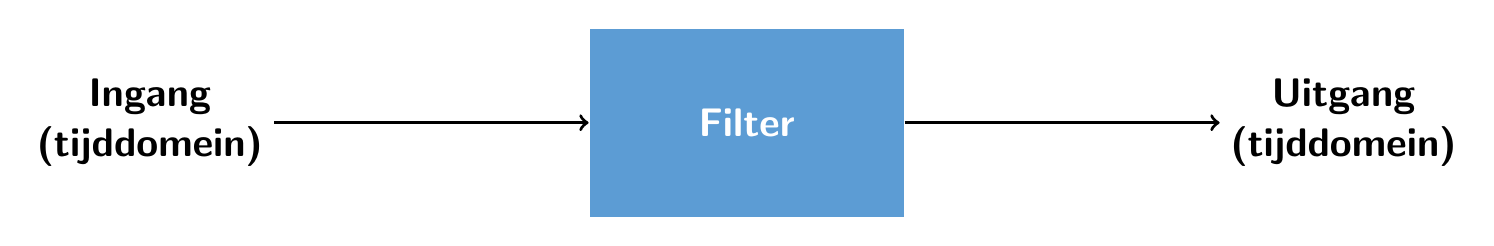
\begin{tikzpicture}[font=\sffamily\Large\bfseries, scale=2]
   \definecolor{babyblueeyes}{rgb}{0.36, 0.61, 0.83}
   \node [draw,
    color=white,
    fill=babyblueeyes,
    minimum width=4cm,
    minimum height=2.4cm
   ]  (filter) {Filter};
   \draw[<-, very thick] (filter.west) -- ++(-2,0) node[left,align=center]{Ingang\\(tijddomein)};
   \draw[->, very thick] (filter.east) -- ++(2,0) node[right,align=center]{Uitgang\\(tijddomein)}; 
\end{tikzpicture}
\end{document}